%課題研究レジュメテンプレート ver. 1.2

\documentclass[uplatex]{jsarticle}
\usepackage[top=20mm,bottom=20mm,left=20mm,right=20mm]{geometry}
\usepackage[T1]{fontenc}
\usepackage{txfonts}
\usepackage{wrapfig}
\usepackage[expert,deluxe]{otf}
\usepackage[dvipdfmx,hiresbb]{graphicx}
\usepackage[dvipdfmx]{hyperref}
\usepackage{pxjahyper}
\usepackage{secdot}

\makeatletter
  \renewcommand{\section}{%
    \if@slide\clearpage\fi
    \@startsection{section}{1}{\z@}%
    {\Cvs \@plus.5\Cdp \@minus.2\Cdp}% 前アキ
    {.5\Cvs \@plus.3\Cdp}% 後アキ
    %{\normalfont\Large\headfont\raggedright}}
    {\normalfont\raggedright}}

  \renewcommand{\subsection}{\@startsection{subsection}{2}{\z@}%
    {\Cvs \@plus.5\Cdp \@minus.2\Cdp}% 前アキ
    {.5\Cvs \@plus.3\Cdp}% 後アキ
    %{\normalfont\large\headfont}}
    {\normalfont}}

  \renewcommand{\subsubsection}{\@startsection{subsubsection}{3}{\z@}%
    {\Cvs \@plus.5\Cdp \@minus.2\Cdp}%
    {\z@}%
    %{\normalfont\normalsize\headfont}}
    {\normalfont}}
\makeatother
%ここから上を編集する必要はない.





\title{\vspace{-14mm}ドローンによる認知症高齢者の徘徊対策}
\author{PMコース 矢吹研究室 1442037 加藤 健弥}
\date{}%日付を入れる必要はない.
\pagestyle{empty}%ページ番号は振らない.
\begin{document}
\maketitle





\section{研究の背景}

%\begin{wrapfigure}[行数]{r}{幅}%行数はオプションだが,調整しないとうまくいかない.
\begin{wrapfigure}[12]{r}{8cm}
\vspace*{-\intextsep}
%\includegraphics[width=図の幅,clip]{ファイル名}\label{参照用ラベル}
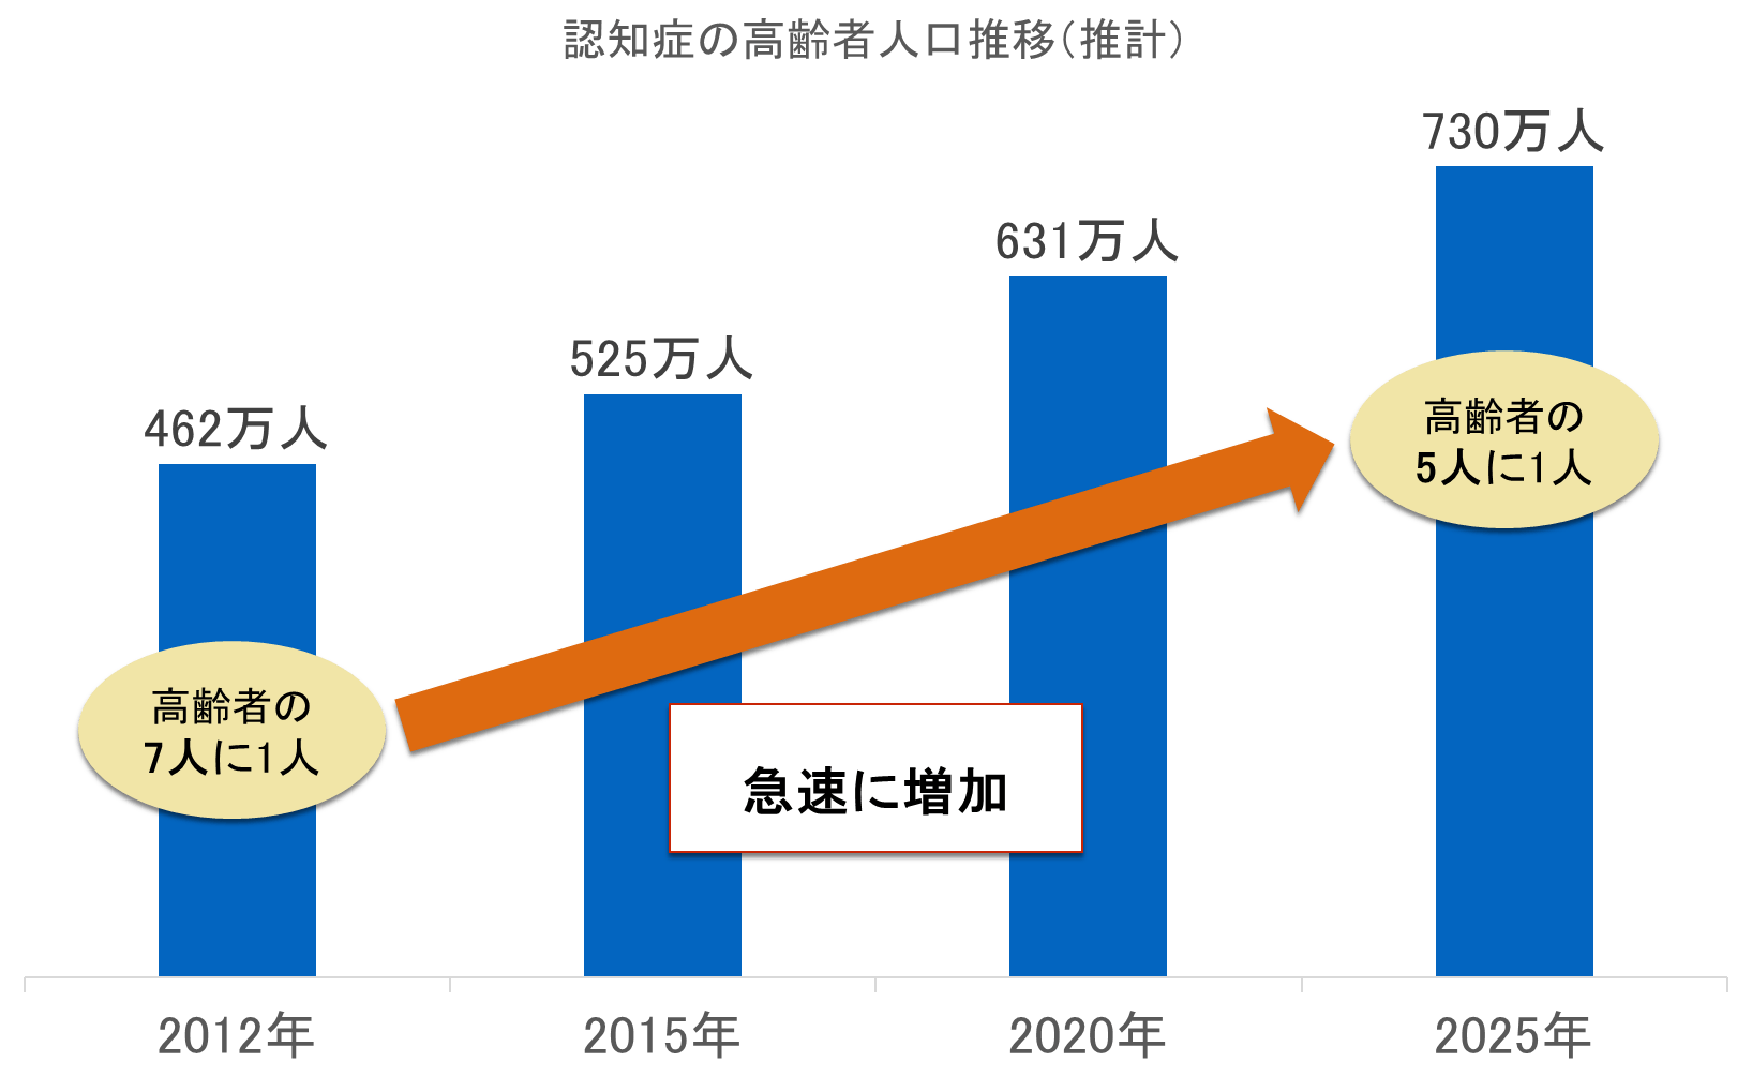
\includegraphics[width=8cm,clip]{ninnti1.pdf}
\caption{認知症の高齢者人口の将来推計に関する研究速報値\cite{self}}\label{サンプル図}
\end{wrapfigure}

私は介護の問題を解決するSI-Lab(Society implementation laboratory)というプロジェクトに取り組んでいる.その理由は2つある.

1つ目の理由として,高齢化社会に向かっている日本という現実がある.その中で認知症高齢者の数も増えており,図1を見てもわかるように2012年の段階で認知症患者の数は推計462万人で高齢者の約7人に1人.今後はさらに増加していき2025年には700万人前後に到達し,65歳以上の高齢者の約5人に1人が認知症患者という予測が立てられている\cite{self}.
認知症高齢者の徘徊行為による行方不明の事案は当然増加しており,年間約1万人が行方不明になっているということが現状である\cite{self1}.
この問題に対して若い世代の我々が持っている技術を用いて貢献できないかと考える.

2つ目の理由として,このプロジェクトがデザイン学科,未来ロボティクス学科,プロジェクトマネジメント学科の3学科合同であり,学んできたことが違う人たちと取り組むことで新しい視点から見ることができるのではないかと考えたためである.


このSI-Lab(Society implementation laboratory)というプロジェクトを行うことで認知症高齢者の問題を3学科の違う視点から解決するための方法を見つけてビジネスとして活かすことができるのではないかと考えた.
 
 

\section{研究の目的}
 
本研究では認知症高齢者への理解を深めて,現代にある技術で問題解決に取り組む.

3学科合同でプロジェクトを取り組み,それをビジネスコンテストに提出して実際にビジネスとして通用するのか確かめる.

実際に介護関係者の方々の前で最終発表を行い,介護の視点から評価をもらう.

\section{プロジェクトマネジメントとの関連}

以下の2つが当てはまる.
\begin{enumerate}
\item コミュニケーション・マネジメント.他学科間によるプロジェクトでは各々が学んできたことが違うため会議の回数を増やす必要性がでてくる.そこで会議ができないことによるプロジェクトの遅延をなくすために休み中でも会議が行えるようにSkypeを使うことで回数を増やす.また集まれないメンバーがいても会議の内容を議事録に記録して共有する.

\item コスト・マネジメント.ビジネスプランを作成する際に事業採算を見積もる必要があるため,ボトムアップ見積もりを行う.
\end{enumerate}



\section{研究の方法}

以下のような順番で研究を進める.
\begin{enumerate}
\item SI-Lab(Society implementation laboratory)に参加し,デザイン学科,未来ロボティクス学科,プロジェクトマネジメント学科の3学科合同でチームを組む.

\item 介護施設に訪問して調査の実施する.

\item 調査から意見を出し合いアイデアを固める.

\item キャンパスベンチャーグランプリというビジネスプランコンテストにビジネスプランの資料を作成して応募する.

\item 実際に介護の現場などで働いている方々を交えた中間発表を行い,介護の視点から意見をもらう.

\item Nikon CORPORATE ACCELERATOR PROGRAMというビジネスプランコンテストにビジネスプランの資料を作成して応募する.

\item 実際に必要なものを揃えてプロトタイプを作成する.

\item 実際に介護の現場などで働いている方々を交えた最終発表する.
\end{enumerate}










\section{現在の進捗状況}

%\begin{wrapfigure}[行数]{r}{幅}%行数はオプションだが,調整しないとうまくいかない.
\begin{wrapfigure}[13]{r}{8cm}
\vspace*{-\intextsep}
%\includegraphics[width=図の幅,clip]{ファイル名}\label{参照用ラベル}
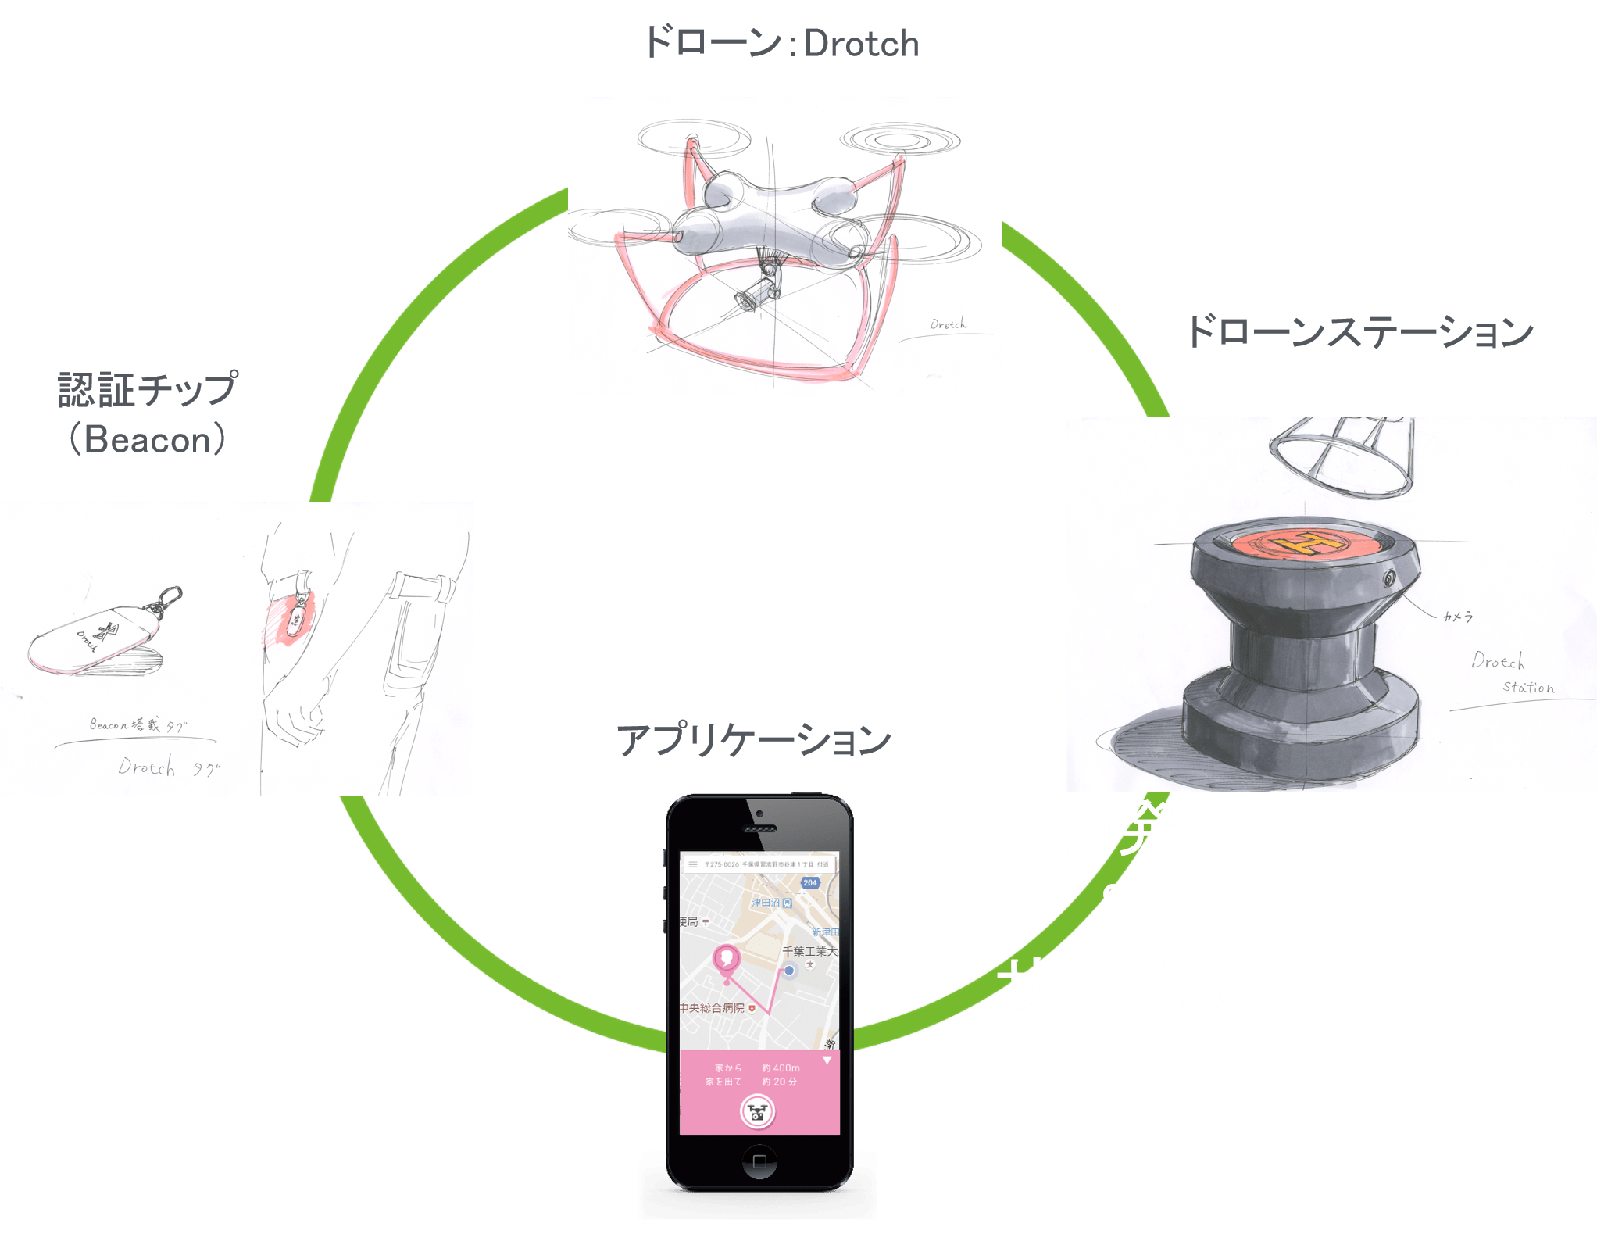
\includegraphics[width=8cm,clip]{SI-Lab1.pdf}
\caption{ドローン,ドローンステーション,タグ,アプリケーションの4つを使った徘徊対策の製品}\label{サンプル図}
\end{wrapfigure}
デザイン学科1名,未来ロボティクス学科1名,プロジェクトマネジメント学科2名のチームを組んで介護施設への調査を実施した.調査では認知症高齢者と実際に話したり触れ合いをすることで理解を深めるとともに問題点を把握した.

調査結果から意見を出し合い,外出した認知症高齢者のタグの有無で知らせ,GPSとカメラを積んでいるドローンで追跡し,アプリケーションで場所を把握するという製品案(図2)が生まれた.図2をもとにキャンパスベンチャーグランプリのビジネスプランの資料を作成し,応募したが落選してしまった.

ビジネスプランを実際に介護の現場などで働いている方々を交えた中間発表を行い,意見をもらった.

もらった意見をブラッシュアップしてNikon CORPORATE ACCELERATOR PROGRAMのビジネスプランコンテストに資料を提出することになった.


\section{今後の計画}

以下のように研究を進める計画である.

\begin{enumerate}
\item Nikon CORPORATE ACCELERATOR PROGRAMにビジネスプランを作成し,期限内に提出する.

\item ドローンのカメラを使って対象を追跡するプログラムのプロトタイプを作成する.

\item ドローンと連携するカメラ映像の取得とGPSで場所を把握するAndroidアプリケーションのプロトタイプを作成する.

\item 実際に介護の現場などで働いている方々を交えた最終発表を行い,介護の視点から評価をもらう.
\end{enumerate}


\bibliographystyle{junsrt}
\bibliography{biblio}%「biblio.bib」というファイルが必要.

\end{document}